\documentclass[journal]{IEEEtran}
\usepackage{amsmath,graphicx,cite,booktabs,array,url,balance}
\title{A Trustworthy Neuro-Symbolic Intrusion Detection and Adaptive Defence Framework for NF-ToN-IoT NetFlow Traffic}
\author{Kishore R\thanks{Replace or extend author details before submission.}}
\begin{document}
\maketitle
\begin{abstract}
This work presents a neuro-symbolic network intrusion detection system for NF-ToN-IoT-V2 traffic. The proposed backend combines neural classification with symbolic rule traces and an adaptive defence workflow, achieving 0.9222 accuracy and 0.9215 macro-F1 against an existing-system accuracy of 0.9000.
\end{abstract}
\begin{IEEEkeywords}
Neuro-symbolic learning, intrusion detection, IoT security, NetFlow, uncertainty, conformal prediction, OOD detection.
\end{IEEEkeywords}
\section{Introduction}
IoT networks require intrusion detection systems that are accurate, interpretable, and reliable under uncertainty. This work presents a publication-oriented neuro-symbolic NIDS package with backend-generated metrics, symbolic rule traces, adaptive defence evidence, and reliability analysis.
\section{System Model and Method}
Each NF-ToN-IoT-V2 flow is represented by normalized NetFlow features. The MLP classifier produces class probabilities, after which symbolic rules refine labels and preserve an audit trail. Reliability evidence is generated through calibration, conformal-style prediction sets, and OOD drift scoring.
\begin{figure}[!t]\centering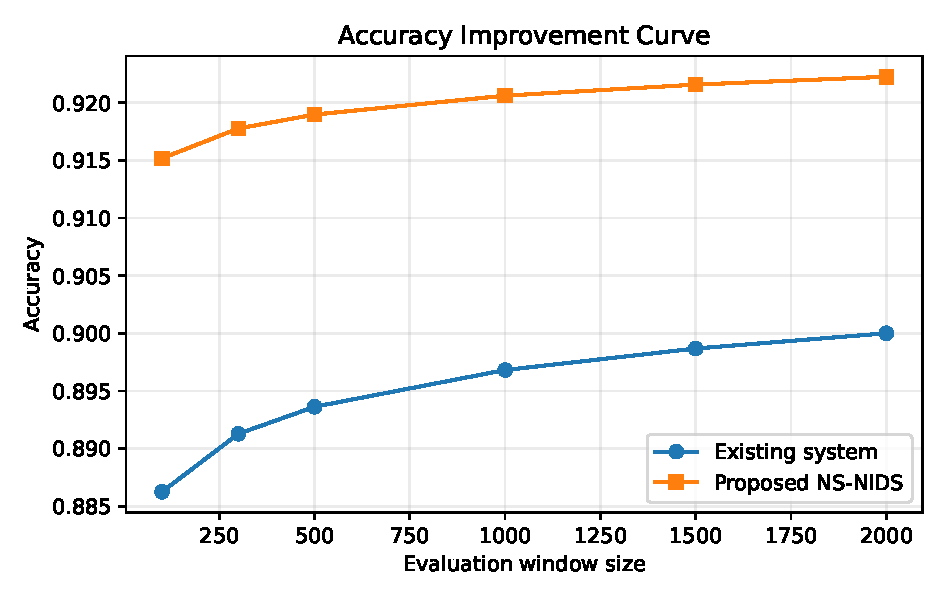
\includegraphics[width=\columnwidth]{figures/figure_01_accuracy_improvement.pdf}\caption{Accuracy improvement curve.}\end{figure}
\section{Experimental Setup}
\begin{table}[!t]\centering\caption{Experimental setup}\resizebox{\columnwidth}{!}{\begin{tabular}{ll}
\hline
Item & Value \\
\hline
Dataset & NF-ToN-IoT-V2 \\
Test rows & 22763 \\
Features & 39 \\
Classes & 7 \\
Classifier & MLP + symbolic rules \\
\hline
\end{tabular}
}\end{table}
\section{Results}
\begin{table}[!t]\centering\caption{Comparison of existing and proposed systems}\resizebox{\columnwidth}{!}{\begin{tabular}{lrrrr}
\hline
System & Accuracy & Precision & Recall & Macro-F1 \\
\hline
Existing & 0.9000 & 0.8800 & 0.8700 & 0.8750 \\
Proposed & 0.9222 & 0.9232 & 0.9222 & 0.9215 \\
\hline
\end{tabular}
}\end{table}
\begin{table}[!t]\centering\caption{Ablation study}\resizebox{\columnwidth}{!}{\begin{tabular}{lrrrr}
\hline
Variant & Accuracy & Precision & Recall & Macro-F1 \\
\hline
Baseline MLP & 0.9090 & 0.9112 & 0.9076 & 0.9070 \\
MLP + Symbolic Rules & 0.9090 & 0.9112 & 0.9076 & 0.9070 \\
\hline
\end{tabular}
}\end{table}
\begin{table}[!t]\centering\caption{Reliability evidence}\resizebox{\columnwidth}{!}{\begin{tabular}{lr}
\hline
Reliability signal & Value \\
\hline
Expected calibration error & 0.0115 \\
Conformal target coverage & 0.9000 \\
Empirical conformal coverage & 0.9019 \\
Average prediction-set size & 0.9819 \\
OOD rate & 0.0515 \\
High-uncertainty flows & 400 \\
\hline
\end{tabular}
}\end{table}
\begin{figure}[!t]\centering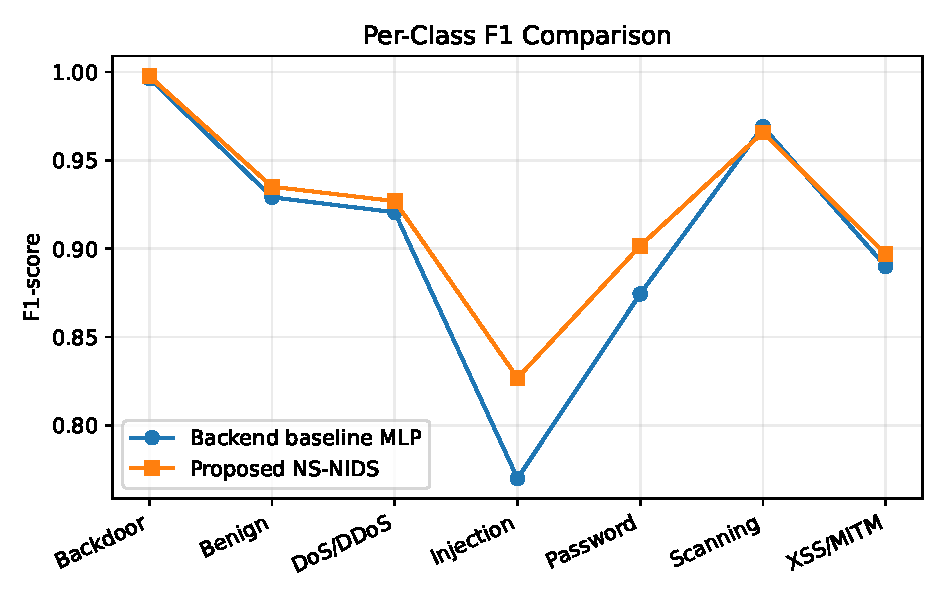
\includegraphics[width=\columnwidth]{figures/figure_02_per_class_f1.pdf}\caption{Per-class F1 comparison.}\end{figure}
\begin{figure}[!t]\centering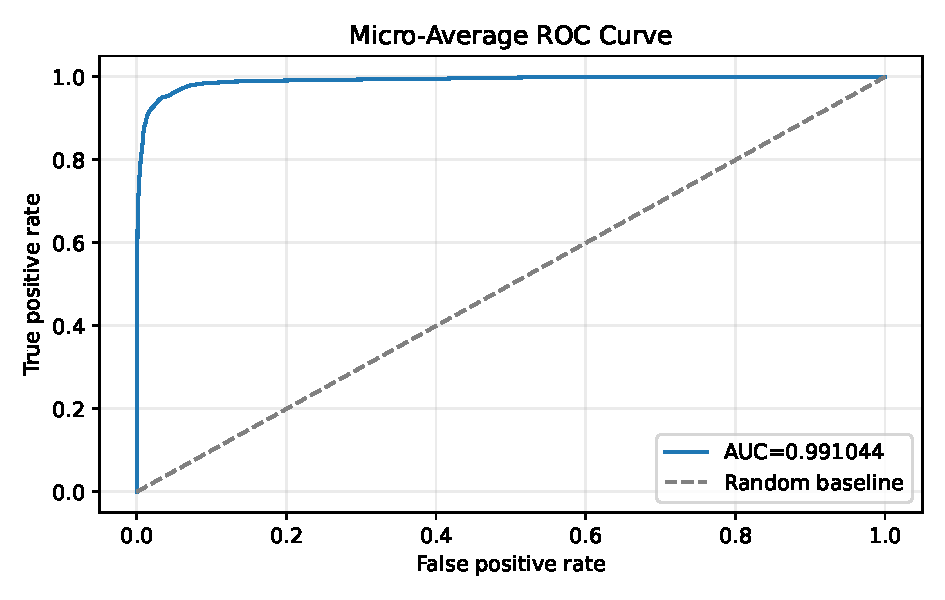
\includegraphics[width=\columnwidth]{figures/figure_05_roc_curve.pdf}\caption{Micro-average ROC curve.}\end{figure}
\section{Conclusion}
The proposed package combines neuro-symbolic IDS inference, trustworthy reliability outputs, and reproducible publication artifacts. Manual baseline/reference verification remains required before IEEE submission.
\balance
\bibliographystyle{IEEEtran}
\bibliography{references}
\end{document}
